\documentclass[12pt]{article}
\usepackage{amssymb, enumerate, amsmath, amsthm}
\usepackage{graphics}
\usepackage{pgfplots}
\usepackage{txfonts}

\newcommand{\problem}[1]{\bigskip \noindent \textbf{Problem #1}}

\theoremstyle{plain}
\newtheorem{theorem}{Theorem}[section]
\newtheorem{corollary}[theorem]{Corollary}
\newtheorem{lemma}[theorem]{Lemma}
\newtheorem{proposition}[theorem]{Proposition}
\newtheorem{conjecture}[theorem]{Conjecture}
\newtheorem{question}{Question}
\newtheorem*{theorem*}{Theorem}
\newtheorem*{example*}{Example}
\newtheorem*{definition*}{Definition}
\newtheorem*{nonexample*}{Non-Example}


\setlength{\oddsidemargin}{0in}
\setlength{\textwidth}{6.5in}
\setlength{\topmargin}{0in}
\setlength{\headheight}{0in}
\setlength{\headsep}{0in}
\setlength{\textheight}{8.7in}
\title{McDonald Exercises, Chapter 2}
\author{Christophe Dethier}
\date{$\substack{\text{Created September 1, 2020}\\\text{Last edited \today}}$}
\begin{document}
\bigskip
\maketitle

Please contact me at christophehldethier@gmail.com with any questions, comments, or corrections.\\

In the following problems, if the ``effective annual interest rate" is $r$, a \$1 investment yields $1 + r$ after 1 year.

\problem{2.1} Suppose XYZ stock has a price of \$50 and pays no dividends. The effective annual interest rate is 10\%. Draw payoff and profit diagrams for a long position in the stock. Verify that profit is 0 at a price in 1 year of \$55.\\

\begin{center}
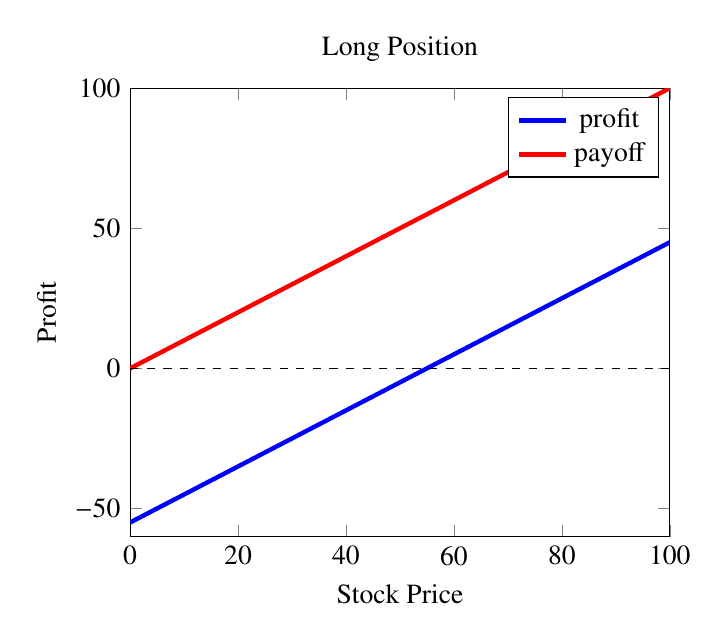
\begin{tikzpicture}
\begin{axis}[
disabledatascaling,
anchor=origin,
xmin=0,xmax=100,
ymin=-60,ymax=100, 
xlabel=Stock Price,
ylabel=Profit,
title=Long Position,
samples=50]
  \addplot[blue, ultra thick, domain=0:100] (x,x-55);
  \addlegendentry{profit};
  \addplot[red,  ultra thick, domain=0:100] (x,x);
  \addlegendentry{payoff};
  \addplot[black, dashed, domain=0:100] (x,0);
\end{axis}
\end{tikzpicture}
\end{center}

As is evident in the graph, the break-even point is a stock price of 55 and a profit of 0.

\problem{2.2} Using the same information as the previous question, draw payoff and profit diagrams for a short position in the stock. Verify that profit is 0 at a price in 1 year of \$55.

\begin{center}
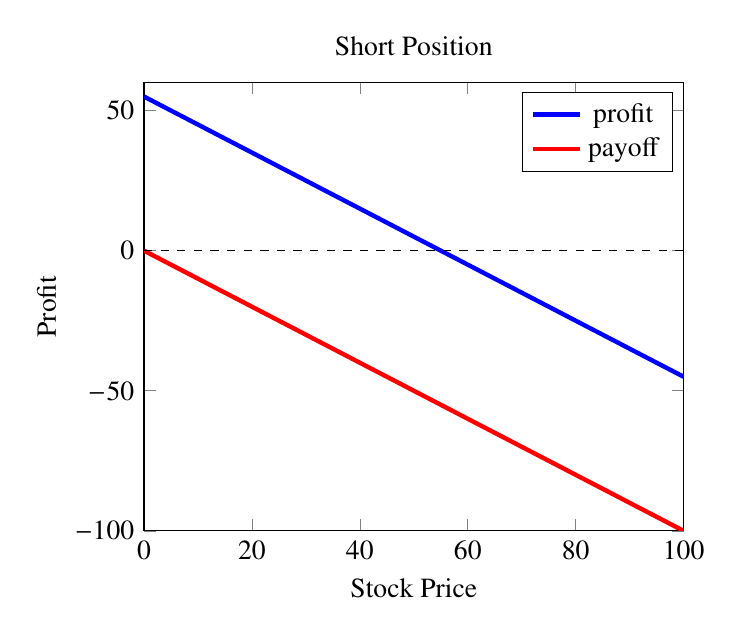
\begin{tikzpicture}
\begin{axis}[
disabledatascaling,
anchor=origin,
xmin=0,xmax=100,
ymin=-100,ymax=60, 
xlabel=Stock Price,
ylabel=Profit,
title=Short Position,
samples=50]
  \addplot[blue, ultra thick, domain=0:100] (x,-x+55);
  \addlegendentry{profit};
  \addplot[red,  ultra thick, domain=0:100] (x,-x);
  \addlegendentry{payoff};
  \addplot[black, dashed, domain=0:100] (x,0);
\end{axis}
\end{tikzpicture}
\end{center}

As is evident in the graph, the break-even point is a stock price of 55 and a profit of 0.

\problem{2.3} What position is the opposite of a purchased call? The opposite of a purchased put?\\

The opposite of a purchased call is a written call. The opposite of a purchased put is a written put. There are other possible answers depending on what one means by ``opposite".

\problem{2.4} 

\begin{enumerate}[(a)]
\item Suppose you enter into a long 6-month forward position at a forward price of \$50. What is the payoff in 6 months for prices of \$40, \$45, \$50, \$55, and \$60?

\begin{center}
Long Forward Position Payoffs\\
\begin{tabular}{l||ccccc}
Stock Price & \$40 & \$45 & \$50 & \$55 & \$60 \\ \hline \hline
Payoff & -\$10 & -\$5 & \$0 & \$5 & \$10
\end{tabular}
\end{center}

\item Suppose you buy a 6-month call option with a strike price of \$50. What is the payoff in 6 months at the same prices for the underlying asset?

\begin{center}
Purchased Call Payoffs\\
\begin{tabular}{l||ccccc}
Stock Price & \$40 & \$45 & \$50 & \$55 & \$60 \\ \hline \hline
Payoff & \$0 & \$0 & \$0 & \$5 & \$10
\end{tabular}
\end{center}

\item Comparing the payoffs of parts (a) and (b), which contract should be more expensive (i.e., the long call or long forward)? Why?

The long call should be more expensive, because the expected profit from the purchased call is positive, which the expected profit from the long forward is \$0. Or to put it another way, it's impossible to have a negative payoff with a purchased call.
\end{enumerate}

\problem{2.5}
\begin{enumerate}[(a)]
\item Suppose you enter into a short 6-month forward position at a forward price of \$50. What is the payoff in 6 months for the prices of \$40, \$45, \$50, \$55, and \$60?

\begin{center}
Short Forward Position Payoffs\\
\begin{tabular}{l||ccccc}
Stock Price & \$40 & \$45 & \$50 & \$55 & \$60 \\ \hline \hline
Payoff & \$10 & \$5 & \$0 & -\$5 & -\$10
\end{tabular}
\end{center}

\item Suppose you buy a 6-month put option with a strike price of \$50. What is the payoff in 6 months at the same prices for the underlying asset?

\begin{center}
Purchased Put Payoffs\\
\begin{tabular}{l||ccccc}
Stock Price & \$40 & \$45 & \$50 & \$55 & \$60 \\ \hline \hline
Payoff & \$10 & \$5 & \$0 & \$0 & \$0
\end{tabular}
\end{center}

\item Comparing the payoffs of parts (a) and (b), which contract should be more expensive (i.e. the long put or the short forward)? Why?

The long put should be more expensive, because the expected profit from the purchased put is positive, which the expected profit from the short forward is \$0. Or to put it another way, it's impossible to have a negative payoff with a purchased put.
\end{enumerate}

\problem{2.6} A default-free zero-coupon bond costs \$91 and will pay \$100 at maturity in 1 year. What is the effective annual interest rate? What is the payoff diagram for the bond? The profit diagram?\\

The effective annual interest rate is
\[
\frac{100}{91} - 1 = 9.89\%.
\]
The payoff and profit diagrams are horizontal lines crossing the profit axis at \$100 and \$9, respectively.

\problem{2.7} Suppose XYZ stock pays no dividends and has a current price of \$50. The forward price for delivery in 1 year is \$55. Suppose the 1-year effective annual interest rate is 10\%. 

\begin{enumerate}[(a)]
\item Graph the payoff and profit diagrams for a forward contract on XYZ stock with a forward price of \$55.

\begin{center}
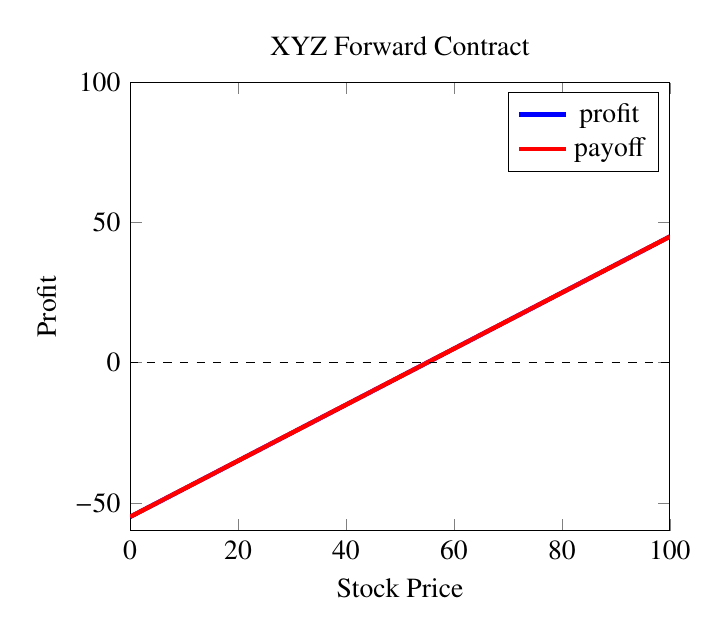
\begin{tikzpicture}
\begin{axis}[
disabledatascaling,
anchor=origin,
xmin=0,xmax=100,
ymin=-60,ymax=100, 
xlabel=Stock Price,
ylabel=Profit,
title=XYZ Forward Contract,
samples=50]
  \addplot[blue, ultra thick, domain=0:100] (x,x-55);
  \addlegendentry{profit};
  \addplot[red,  ultra thick, domain=0:100] (x,x-55);
  \addlegendentry{payoff};
  \addplot[black, dashed, domain=0:100] (x,0);
\end{axis}
\end{tikzpicture}
\end{center}

\item Is there any advantage to investing in the stock or the forward contract? Why?

In some sense there is no advantage, as we can see the payoff and profit diagrams from this problem and {Problem 2.1} are identical. I suppose there may be advantage in the forward option if you have an investment that you think could beat the 10\% interest rate.

\item Suppose XYZ paid a dividend of \$2 per year and everything else stayed the same. Now is there any advantage to investing in the stock or the forward contract? Why?

Now there is an advantage to investing in the stock, as you obtain the \$2 dividend that way that you wouldn't otherwise.

\end{enumerate}

\problem{2.8} Suppose XYZ stock pays no dividends and has a current price of \$50. The forward price for delivery in one year is \$53. \emph{If} There is no advantage to buying either the stock or the forward contract, what is the 1-year effective interest rate?\\

The effective annual interest rate is then
\[
\frac{53}{50} - 1 = 6\%.
\]

\problem{2.9} An \emph{off-market} forward contract is a foward where either you have to pay a premium or you receive a premium for entering into the contract. (With a standard forward contract, the premium is zero.) Suppose the effective annual interest rate is 10\% and the S\&R index is 1000. Consider 1-year forward contracts.

\begin{enumerate}[(a)]
\item Verify that if the forward price is \$1100, the profit diagrams for the index and the 1-year forward are the same.

\begin{center}
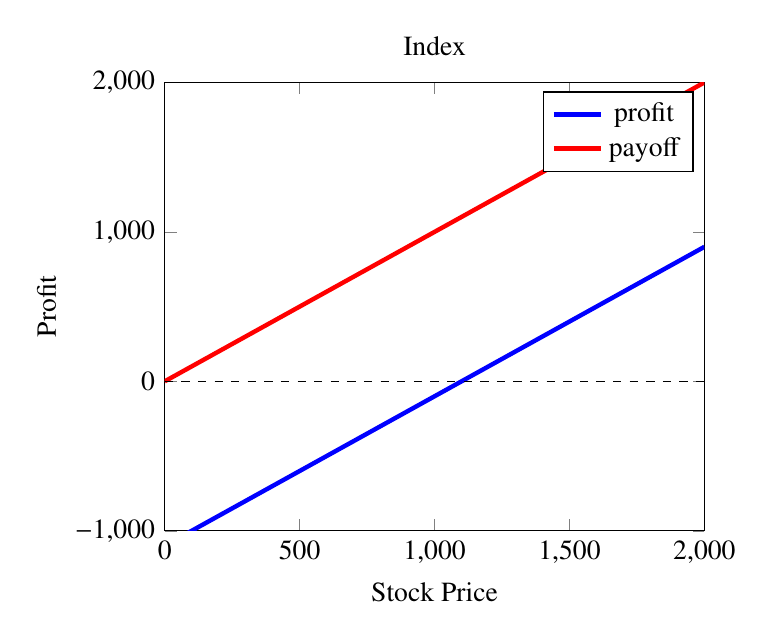
\begin{tikzpicture}
\begin{axis}[
disabledatascaling,
anchor=origin,
xmin=0,xmax=2000,
ymin=-1000,ymax=2000, 
xlabel=Stock Price,
ylabel=Profit,
title=Index,
samples=50]
  \addplot[blue, ultra thick, domain=0:2000] (x,x-1100);
  \addlegendentry{profit};
  \addplot[red,  ultra thick, domain=0:2000] (x,x);
  \addlegendentry{payoff};
  \addplot[black, dashed, domain=0:2000] (x,0);
\end{axis}
\end{tikzpicture}
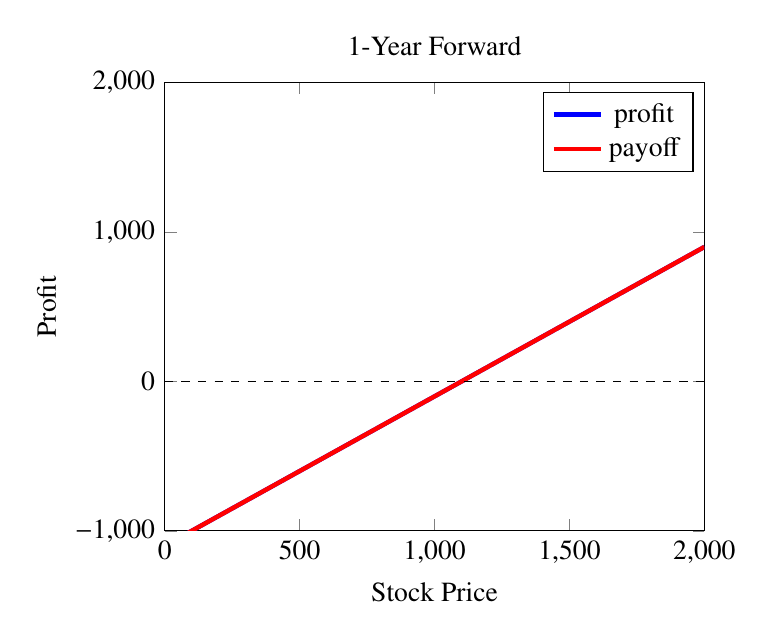
\begin{tikzpicture}
\begin{axis}[
disabledatascaling,
anchor=origin,
xmin=0,xmax=2000,
ymin=-1000,ymax=2000, 
xlabel=Stock Price,
ylabel=Profit,
title=1-Year Forward,
samples=50]
  \addplot[blue, ultra thick, domain=0:2000] (x,x-1100);
  \addlegendentry{profit};
  \addplot[red,  ultra thick, domain=0:2000] (x,x-1100);
  \addlegendentry{payoff};
  \addplot[black, dashed, domain=0:2000] (x,0);
\end{axis}
\end{tikzpicture}
\end{center}
As we can see, the two profit diagrams are identical.

\item Suppose you are offered a long forward contract at a forward price of \$1200. How much would you need to be paid to enter into this contract?\\

I would need to be paid \$100 discounted with a 10\% effective annual interest rate;
\[
\frac{100}{1.1} = \$90.91.
\]

\item Suppose you are offered a long forward contract at a forward price of \$1000. How much would you be willing to pay to enter into this forward contract?

I would be willing to pay \$100 discounted with a 10\% effective annual interest rate;
\[
\frac{100}{1.1} = \$90.91
\]
\end{enumerate}

\problem{2.10} For Figure 2.6, verify the following:
\begin{enumerate}[(a)]
\item The S\&R index price at which the call option diagram intersects the $x$-axis is \$1095.68.\\

The S\&R index price at which the call option diagram intersects the $x$-axis is the S\&R index price which gives the call option a return of \$0. As the future value of the premium is \$95.68, the strike price is \$1000, and the call returns the value of the S\&R index, we see that when the S\&R index price is \$1095.68 the profit of the call option is \$0.

\item The S\&R index price at which the call option and forward contract have the same profit is \$924.32.\\

The horizontal portion of the call option gives a profit of -\$95.68, so we need to find where the forward contract returns a profit of -\$95.68. Since the forward contract returns the value of the S\&R index minus \$1020, we see that the profit of the forward contract will be -\$95.68 when the S\&R index price is \$924.32.

\end{enumerate}

\problem{2.11} For Figure 2.8, verify the following:
\begin{enumerate}[(a)]
\item The S\&R index price at which the put option diagram intersects the $x$-axis is \$924.32\\

The put option intersect the $x$-axis when the profit of the put option is \$0. Since the future value of the premium is \$75.68, we see that the put has a profit of \$0 when the return from selling the index is \$75.68. Since the strike price is \$1000, the S\&R index price must be \$924.32.

\item The S\&R index price at which the put option and forward contract have the same profit is \$1095.68.\\

Since the horizontal portion of the put option diagram gives a profit of -\$75.68, we need to find the S\&R index price which gives the short S\&R index forward a profit of -\$75.68. Since the forward option has a strike price of \$1020, the S\&R index price must be \$1095.68 to return a profit of \$0.
\end{enumerate}

\problem{2.12} For each entry in Table 2.5, explain the circumstances in which the maximum gain or loss occurs.\\

The long forward has maximum loss when the stock has a value of \$0 when the sale occurs. The long forward has maximum gain when the price of the stock rises sharply. There is no bound for this.

The short forward has maximum loss when the stock price rises sharply. There is no bound for this. The short forward has maximum gain when the stock has a value of \$0 when the sale occurs.

The long call has maximum loss when the stock has a value less than strike price at the time of sale. The long call has a maximum gain when the stock price rises sharply. There is no bound to this.

The short call has maximum loss when the stock price rises sharply. There is no upper bound for this. The short call has maximum gain when the stock has a value less than the strike price at the time of sale.

The long put has maximum loss when increase in stock value exceeds the premium at the time of sale. The long put has maximum gain when the stock has a value of \$0 at the time of sale.

The short put has maximum loss when the stock has a value of \$0 at the time of sale. The short put has maximum gain when the increase in stock value exceeds the premium at the time of sale.

\problem{2.13} Suppose the stock price is \$40 and the effective annual interest rate is 8\%. 
\begin{enumerate}[(a)]
\item Draw on a single graph payoff and profit diagrams for the following options:
\begin{enumerate}[(i)]
\item 35-strike call with a premium of \$9.12.
\item 40-strike call with a premium of \$6.22.
\item 45-strike call with a premium of \$4.08.
\end{enumerate}

\begin{center}
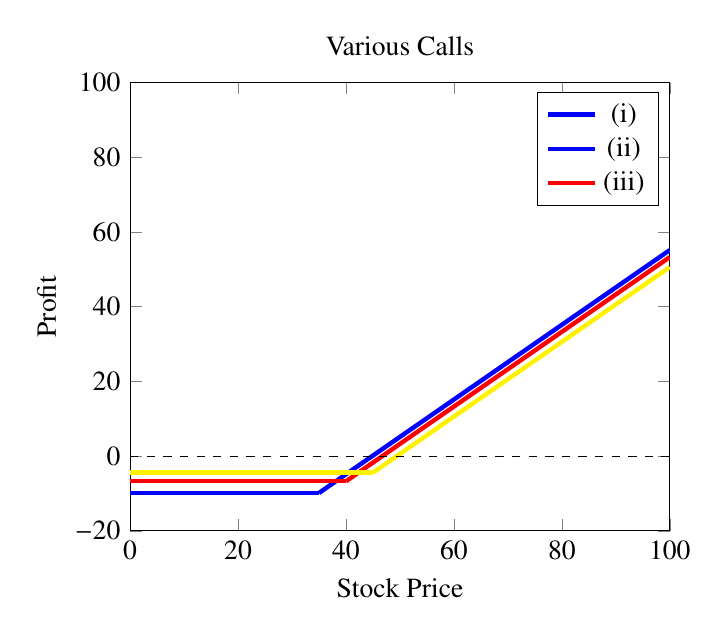
\begin{tikzpicture}
\begin{axis}[
disabledatascaling,
anchor=origin,
xmin=0,xmax=100,
ymin=-20,ymax=100, 
xlabel=Stock Price,
ylabel=Profit,
title=Various Calls,
samples=50]
  \addplot[blue, ultra thick, domain=0:35] (x,-9.85);
  \addplot[blue, ultra thick, domain=35:100] (x,x-44.85);
  \addlegendentry{(i)};
  \addplot[red, ultra thick, domain=0:40] (x,-6.72);
  \addplot[red, ultra thick, domain=40:100] (x,x-46.72);
  \addlegendentry{(ii)};
  \addplot[yellow, ultra thick, domain=0:45] (x,-4.41);
  \addplot[yellow, ultra thick, domain=45:100] (x,x-49.41);
  \addlegendentry{(iii)};
  \addplot[black, dashed, domain=0:100] (x,0);
\end{axis}
\end{tikzpicture}
\end{center}
Note that we use the future values of the premiums in this profit diagram (if it isn't easy to see in the picture).

\item Consider your payoff diagram with all three options graphed together. Intuitively, why should the option premium decrease with the strike price?\\

If the strike price is higher you are paying more for the purchase of the stock. Therefore the premium should be lower to compensate for this. Otherwise a higher strike price would only be a worse deal.

\end{enumerate}

\problem{2.14} Suppose the stock price is \$40 and the effective annual interest rate is 8\%. 
\begin{enumerate}[(a)]
\item Draw payoff and profit diagrams for the following options:
\begin{enumerate}[(i)]
\item 35-strike put with a premium of \$1.53.
\item 40-strike put with a premium of \$3.26
\item 45-strike put with a premium of \$5.75
\end{enumerate}

\begin{center}
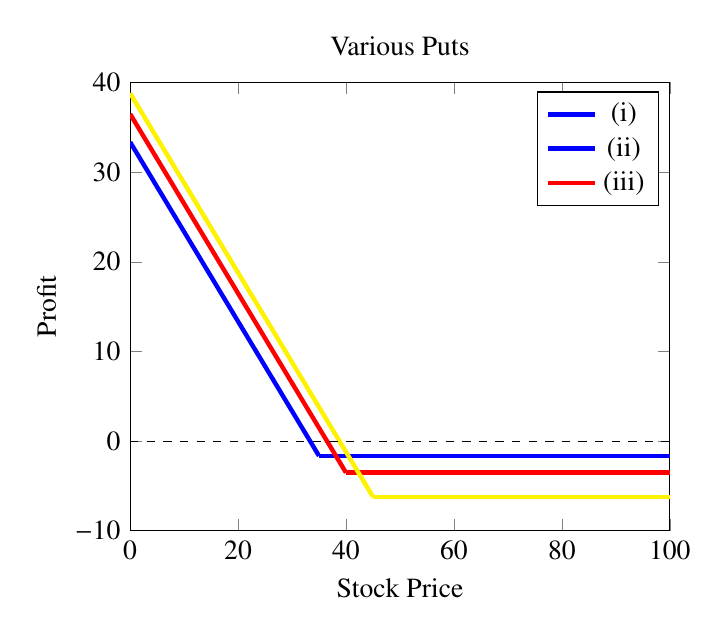
\begin{tikzpicture}
\begin{axis}[
disabledatascaling,
anchor=origin,
xmin=0,xmax=100,
ymin=-10,ymax=40, 
xlabel=Stock Price,
ylabel=Profit,
title=Various Puts,
samples=50]
  \addplot[blue, ultra thick, domain=35:100] (x,-1.65);
  \addplot[blue, ultra thick, domain=0:35] (x,33.35-x);
  \addlegendentry{(i)};
  \addplot[red, ultra thick, domain=40:100] (x,-3.52);
  \addplot[red, ultra thick, domain=0:40] (x,36.48-x);
  \addlegendentry{(ii)};
  \addplot[yellow, ultra thick, domain=45:100] (x,-6.21);
  \addplot[yellow, ultra thick, domain=0:45] (x,38.79-x);
  \addlegendentry{(iii)};
  \addplot[black, dashed, domain=0:100] (x,0);
\end{axis}
\end{tikzpicture}
\end{center}
Note that we use the future values of the premiums in this profit diagram (if it isn't easy to see in the picture).

\item Consider your payoff diagram with all three options graphed together. Intuitively, why should the option premium increase with the strike price?\\

If the strike price increases, you sell for a higher price in the event of a sale. Therefore, the premium should be higher to compensate for this. Otherwise the higher strike price would always be a better deal.
\end{enumerate}

\problem{2.15} The profit calculation in the chapter assumes that you borrow at a fixed interest rate to finance investments. An alternative way to borrow is to short-sell stock. What complications would arise in calculating profit if you financed a \$1000 S\&R index investment by shorting IBM stock, rather than by borrowing \$1000?\\

The outcome of the short-sale is variable. You could graph this as a surface, thinking of profit as dependent on the resulting IBM stock and the resulting S\&R index price.

\problem{2.16} Construct a spreadsheet that permits you to compute payoff and profit for a short and long stock, a short and long forward, and purchased and written puts and calls. The spreadsheet should let you specify the stock price, forward price, interest rate, option strikes, and option premiums. Use the spreadsheet's max function to compute option payoffs.\\

This spreadsheet can be found at
\begin{verbatim}
McDonald_Chapter2.xls
\end{verbatim}
In the same folder as this file.

\end{document}